\chapter{Captura XADC y memoria FIFO}
\label{section:xadc_fifo}


Como se ha introducido anteriormente, en este capítulo se definirá el proceso de captura y conversión de una señal de entrada triangular y el posterior almacenamiento de la misma en una memoria FIFO. En la Figura \ref{fig:xadc_fifo} se muestra el diseño de los bloques necesarios para esta fase y la definición de sus correspondientes puertos de entrada y salida.

\vspace{3mm}

\begin{figure}[h]
    \centering
    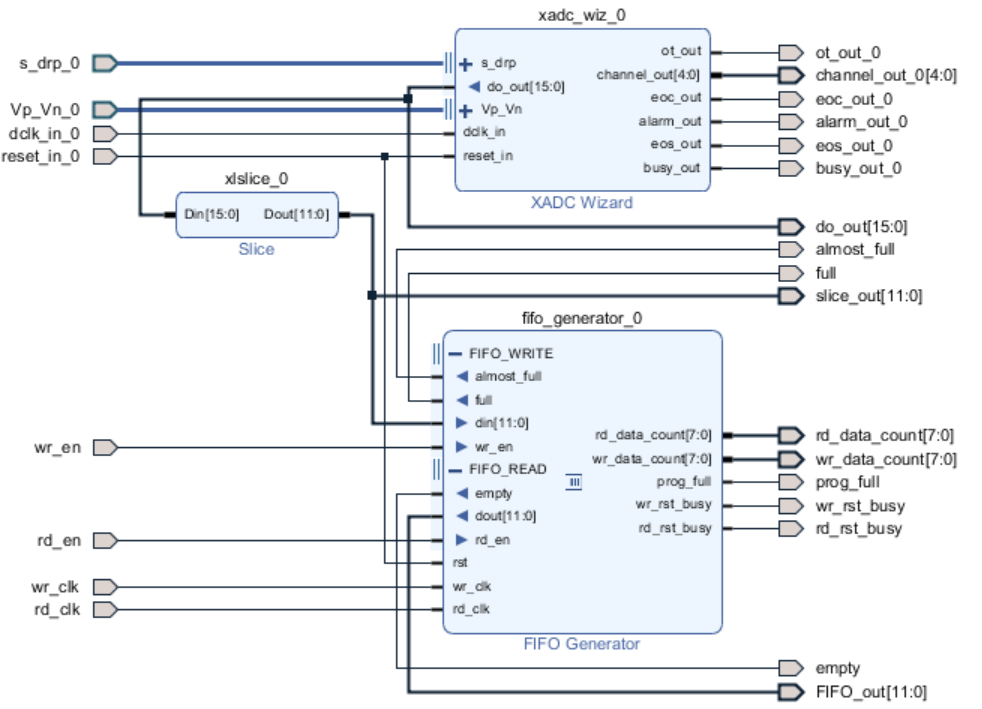
\includegraphics[width=0.9\textwidth]{img/diseno/xadc_fifo.PNG}
    \caption{Diseño del bloque XADC+FIFO}
    \label{fig:xadc_fifo}
\end{figure}
    
\vspace{3mm}

\section{Obtención de los datos convertidos del ADC}

\subsection{Configuración del XADC}

En primer lugar, teniendo en cuenta que nuestro puesto de laboratorio es el 8, se debe generar a la entrada una señal triangular con un valor de frecuencia igual a 13KHz y que opere en un rango de valores de tensión entre 0 y 0.596 voltios. Los valores que toma en cada instante temporal serán definidos en el fichero design.txt, el cual tendrá que ser importado al proyecto para llevar a cabo la conversión.

Como se puede ver en la Figura \ref*{fig:design} se definen valores de tensión para dos entradas (VP y VN), que corresponden a las entradas analógicas diferenciales del XADC. Por simplificación, se configura el valor absoluto de tensión para la entrada positiva (VP) y un valor nulo para la negativa (VN). 

\vspace{3mm}

\begin{figure}[h]
    \centering
    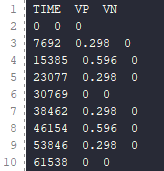
\includegraphics[width=0.3\textwidth]{img/diseno/design.PNG}
    \caption{Valores de tensión (V) de la señal triangular extraídos de design.txt}
    \label{fig:design}
\end{figure}
    
\vspace{3mm}

%el escalon max del ADC = (3/4096)/2 -> el error max, la precisión tiene que ser menor que el error, si no se pierde resolución.
%en vp_vn se pone una precisión segun esto
%0.000366 -> precisión de 10e-4, tensiones de 4 decimales.

El XADC se configura en modo continuo y con un único canal de entrada para capturar las muestras, por lo que se ha seleccionado el canal 3 para registrar el valor convertido de tensión (\textit{s\_drp\_daddr}). La conversión se realizará a una velocidad de 1 MS/seg con un reloj de 52 MHz y se establecerá un tiempo de adquisición igual a 4 para que la señal de captura sea estable.

%hablar de la configuración del xadc
%poner foto del esquema de la documentación
%hablar del 192mhz
%repetir capturas
%meter codigo


\subsection{Simulación de la señal de entrada}

Una vez configurado el bloque IP XADC se procede a simular la conversión de la señal de entrada. En la figura \ref{fig:xadc} se puede visualizar cómo se obtiene la salida digital de 16 bits por el puerto \textit{do\_out}.

\vspace{3mm}

\begin{figure}[h]
    \centering
    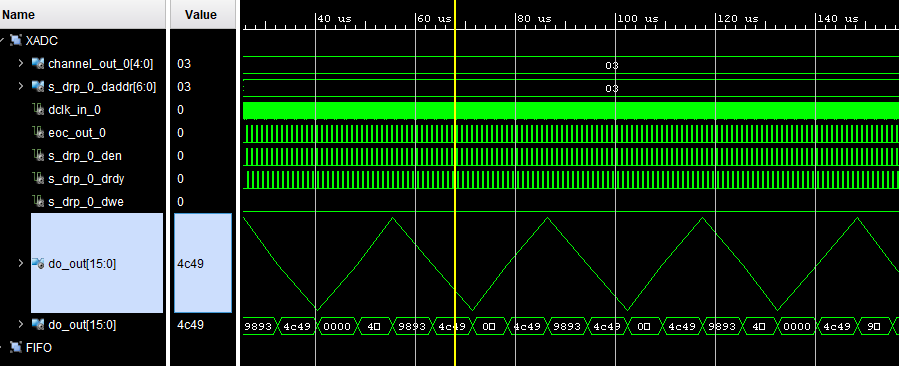
\includegraphics[width=1\textwidth]{img/simu/xadc.PNG}
    \caption{Conversión analógico-digital de la señal triangular de entrada (I)}
    \label{fig:xadc}
\end{figure}

\vspace{3mm}
\pagebreak

Por otro lado, en la Figura \ref{fig:xadc2} se aprecia de una forma más clara los valores que toman cada uno de los puertos del XADC en cada conversión. La señal de fin de conversión \textit{eoc\_out} se activa y como consecuencia, también lo hará la de enable del Puerto de Reconfiguración Dinámico (DRP) \textit{eoc\_out}. 

\vspace{3mm}

\begin{figure}[h]
    \centering
    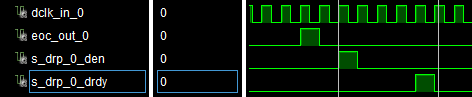
\includegraphics[width=0.7\textwidth]{img/simu/xadc2.PNG}
    \caption{Fin de conversión y dato preparado (III)}
    \label{fig:xadc2}
\end{figure}

\vspace{3mm}

La operación de lectura se completa cuando la señal de dato ready se activa \textit{s\_drp\_drdy}, indicando que se ha sacado el dato a la salida y que se puede proceder a convertir el siguiente.

\vspace{3mm}

\begin{lstlisting}[language=VHDL, style=mystyle, caption={Bucle de conversión de los 200 datos}]
-- frec. conversion aprox 1MS -> frec 52 KHz (modo continuo)
for i in 0 to 200 -- a la espera de 200 datos 
loop     
    -- End of Conversion signal 
    wait until eoc_out_0 <= '1' ; 
    -- Data ready signal for the dynamic reconfiguration port  
    wait until s_drp_0_drdy = '1'; 
end loop;
\end{lstlisting}

\section{Lógica de control de lectura y escritura de los datos de la FIFO}

\subsection{Configuración del bloque FIFO}

El bloque de memoria FIFO almacenará cada uno de los datos capturados por el bloque XADC. Consta de una capacidad de 256 posiciones de 12 bits cada una, por lo que a la entrada del bloque FIFO será precisa la configuración de un bloque auxiliar Slice para transformar los 16 bits de la señal de salida del XADC en sus 12 bits de mayor peso. 

\vspace{3mm}

\begin{figure}[h]
    \centering
    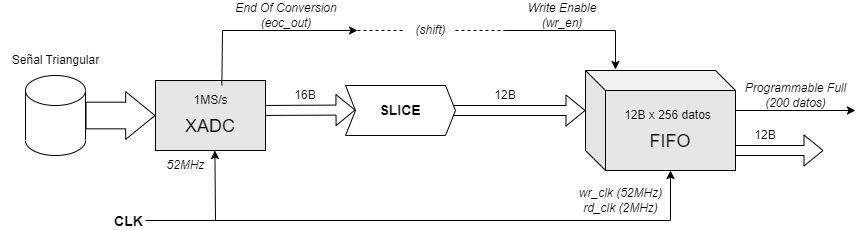
\includegraphics[width=1\textwidth]{img/diseno/xadc_fifo.drawio.PNG}
    \caption{Diseño del bloque XADC+FIFO}
    \label{fig:xadc_fifo}
\end{figure}
    
\vspace{3mm}

Se trata de un paso necesario porque el XADC en el fondo maneja una precisión de 12 bits a la salida. En la Figura \ref*{fig:xadc_fifo} se puede apreciar esta conversión, además de la estructura completa del bloque a implementar.

\vspace{5mm}

\begin{lstlisting}[language=VHDL, style=mystyle, caption={Proceso de escritura}]
process(wr_clk) 
variable reg : std_logic; -- variable para almacenar dato de salida del xadc
begin
if rising_edge(wr_clk) then
    if reset_in_0 = '1' then -- reset XADC = 1
        reg := '0';
        -- Enable signal for the dynamic reconfiguration port
        s_drp_0_den <= '0'; 
    else
        s_drp_0_den <= reg ; -- ENABLE = 1 solo durante un ciclo
        reg := eoc_out_0; -- Se habilita la salida de un nuevo dato 
    end if;
end if;
end process; 

wr_en <= s_drp_0_drdy; -- se escribe en la FIFO nuevo dato 
\end{lstlisting}

\vspace{3mm}

\pagebreak

Entrando en el proceso de escritura, el funcionamiento sería el siguiente: cada vez que exista un nuevo dato proporcionado por el XADC se escribirá en la memoria FIFO de forma continua a 1 MS/s y con un reloj de 52 MHz (\textit{wr\_clk}) hasta llegar a la capacidad máxima.

Una vez la memoria FIFO está llena, comenzará el proceso de lectura de 200 datos a una frecuencia de lectura de 2MHz (\textit{rd\_clk}) mediante la activación de la señal (\textit{rd\_enable}). En este caso, al desear leer un número de datos menor a la capacidad máxima (256), será necesario configurar una señal auxiliar programable (\textit{programable\_full}).

\vspace{5mm}

\begin{lstlisting}[language=VHDL, style=mystyle, caption={Proceso de lectura}]
process(rd_clk) 
file outfile: text is out "FIFO_output.txt"; 
variable line_num: line;
variable opened, finished: std_logic := '0'; 
begin
    file_open (outfile, "FIFO_output.txt", write_mode); 
    if rising_edge(rd_clk) then
        if reset_in_0 = '1' then -- reset XADC = 1
            rd_en <= '0';
        else
            --se comienza a leer la FIFO 
            if prog_full = '1' then 
                rd_en <= '1';
            end if; 
            if empty = '1' then  
                rd_en <= '0';
            end if;
            --proceso de escritura del .txt
            if rd_en = '1' and finished = '0' then 
                write (line_num, FIFO_out);
                writeline(outfile, line_num);
                opened := '1';
            end if;
            --Se finaliza la escritura de .txt tras el primer empty
            if opened = '1' and empty = '1' then 
                finished := '1';
            end if;
        end if;
    end if;
end process;   
\end{lstlisting}

\vspace{3mm}

Adicionalmente, es necesario implementar la escritura de un fichero de salida con los datos almacenados en la FIFO, en el cual cada dato de 12 bits será una nueva línea. Este servirá para simular la lectura de la FIFO desde otro proyecto independiente de Vivado, suponiendo de este modo la entrada del siguiente bloque de mapeado. Se debe limitar la escritura a los primeros 200 datos de salida mediante el uso de variables adicionales (\textit{opened}, \textit{finished}).

\pagebreak

\subsection{Comprobación del bloque FIFO}

En las Figuras \ref{fig:fifo_wr} y \ref{fig:fifo_rd} se pueden visualizar los procesos de escritura y de lectura en la memoria FIFO como se ha descrito en el apartado anterior. A modo de depuración de que se está produciendo un correcto funcionamiento según los tiempos configurados, se añaden a la simulación dos señales de contadores de ciclos de lectura y de escritura.

\vspace{3mm}

\begin{figure}[h]
    \centering
    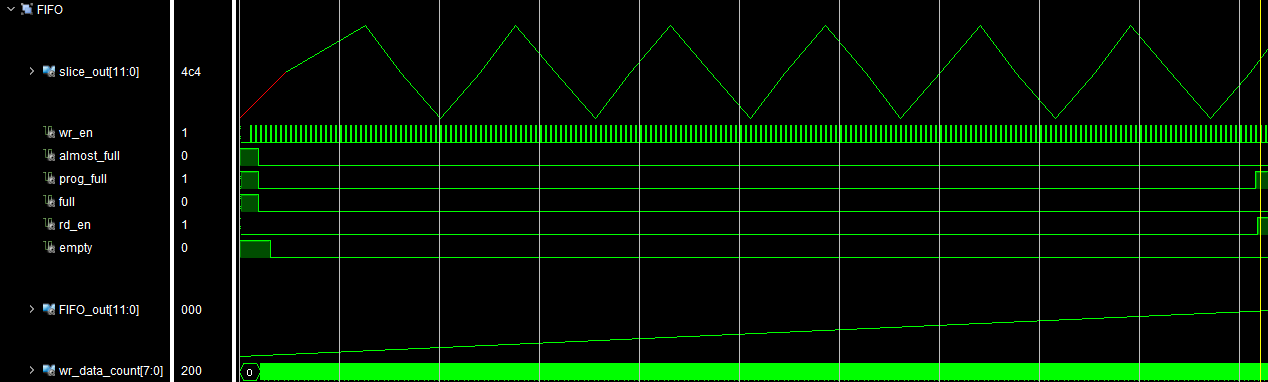
\includegraphics[width=1\textwidth]{img/simu/fifo_wr.PNG}
    \caption{Simulación del proceso de escritura en la memoria FIFO}
    \label{fig:fifo_wr}
\end{figure}
    
\vspace{3mm}

\begin{figure}[h]
    \centering
    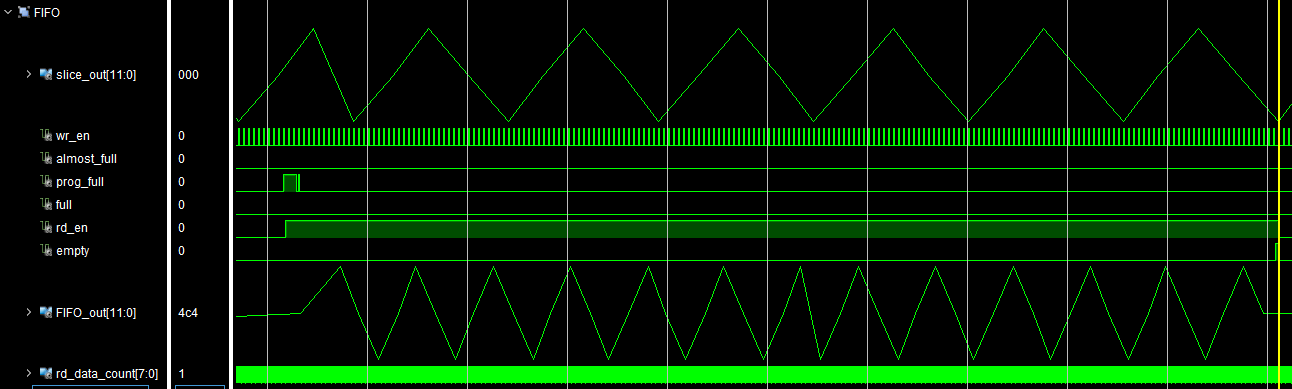
\includegraphics[width=1\textwidth]{img/simu/fifo_rd.PNG}
    \caption{Simulación del proceso de lectura en la memoria FIFO}
    \label{fig:fifo_rd}
\end{figure}
    
\vspace{3mm}

%explicar como esta relacionado con el xadc
%configuración de contadores de lectura y escritura
      
